\chapter{Apresentação da Concedente} % (fold)
\label{chap:Apresentação da Concedente}
Em \cite{CARVALHO:2012} orienta-se aos estagiários tomarem conhecimento do ambiente escolar primeiramente por intermédio da observação e da análise, buscando-se compreender a realidade em que se contra, bem como a relação da unidade escolar com a comunidade, dessa forma, pretende-se estabelecer a vivência pedagógica a partir da tomada de conhecimento de maneira humana e solidarizada.

\section{Caracterização da Unidade} % (fold)
\label{sec:Caracterização da Unidade}
\setlength\intextsep{0pt}
\begin{wrapfigure}[9]{r}{0.5\textwidth}
	\centering
	\label{fig:vista-externa}
	\caption{EEB-GPF: Visão externa.}
	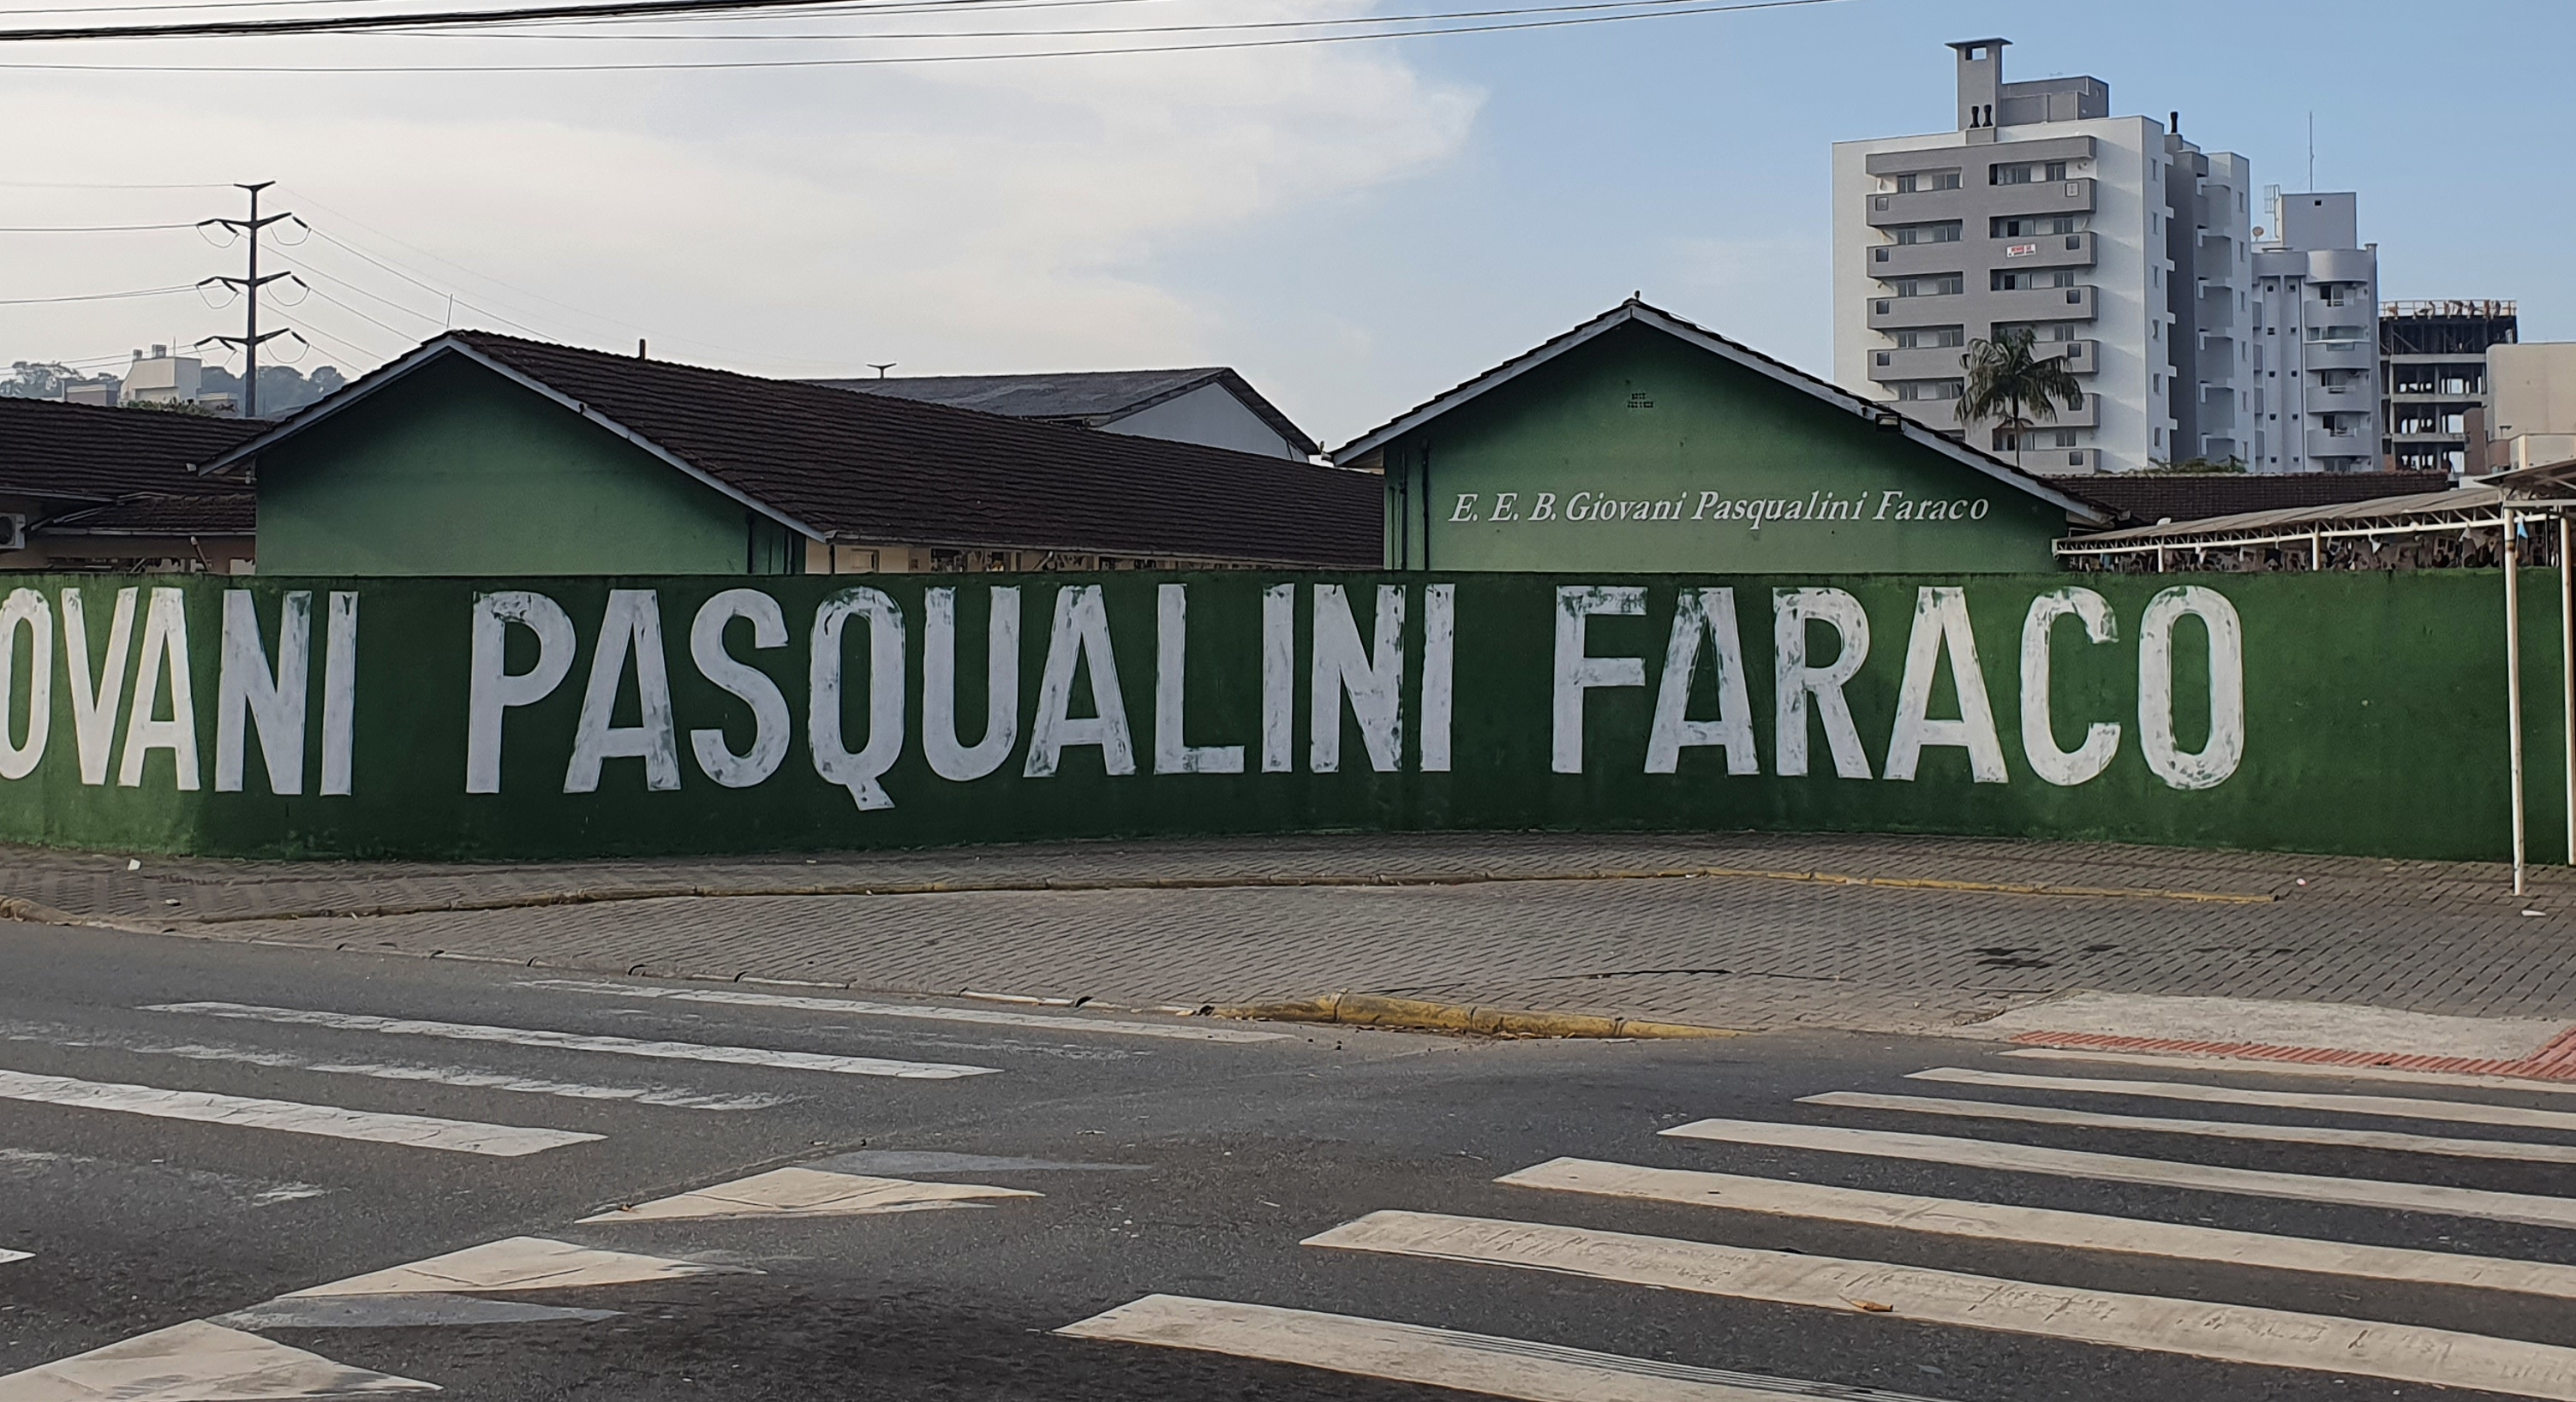
\includegraphics[width=.45\textwidth]{assets/vista-ext01.jpg}
	\legend{Fonte: O autor}
\end{wrapfigure}
A \ac{EEB} \ac{GPF} não se destingue do padrão estrutural das escolas pública de Joinville, tal como outras tantas, mistura-se à paisagem urbana da região, neste caso, a região norte da cidade. Em tinta branca e em caixa alta é lido o nome da escola numa parte do muro e, dessa forma, os muros não apenas lhe conferem \emph{proteção}, mas também referência.

\setlength\intextsep{0pt}
\begin{wrapfigure}[15]{l}{0.5\textwidth}
	\centering
	\label{fig:entr-principal}
	\caption{EEB-GPF: Entrada principal}
	\includegraphics[width=.45\textwidth]{assets/entrada-01.jpg}
	\legend{Fonte: O autor}
\end{wrapfigure} A entrada principal, consiste num portão largo, aberto ao início e final de cada turno, é por onde passam a maioria dos alunos, um segundo portão feito de grade e estreito é visto mais adiante, este da acesso à secretaria. Sempre de clima agradável, bem equipada e limpa, a secretaria é a primeira instância administrativa de que a comunidade tem acesso direto à escola, há sempre alguém de prontidão e não demora muito a atendê-lo. Folhetos no balcão e cartazes colados nos murais, informam as datas e atividades que a escola desenvolve em conjunto com a comunidade. Um caminho estreito e florido, liga a secretaria ao hall onde ficam as salas: do(a) \ac{ATP}, da Direção Geral, e dos Professores.

% section Caracterização da Unidade (end)

\subsection{Histórico} % (fold)
\label{sec:Histórico}
Foi fundada no dia 15 de fevereiro de 1938 (85 anos) sob o nome: \textit{Escola Desdobrada Dona Francisca Quilômetro Cinco}. Encontra-se situada junto à Rua Dona Francisca, número 4957, Bairro Santo Antônio, região norte de Joinville-SC. 

Atualmente têm em seu nome o patrono da instituição: \emph{Giovani Faraco} -- brasileiro, nascido em 05 de abril de 1915, foi professor de latin, português e compositor de músicas para órgãos. O Decreto de n$^\circ$ 10138/70 renomeia a unidade para Grupo Escolar Giovani Pasqualini Faraco e em 08 de junho de 1993, recebe aprovação do Conselho Estadual de Educação para implantar o Ensino Médio através do parecer de n$^\circ$ 117/93, integrando desde então a rede Estadual de Ensino.
% subsection Histórico (end)

\subsection{Infraestrutura} % (fold)
\label{sec:Infraestrutura}

Tem por área construída  $3114,50\m^2$ e outros $13929,25\m^2$ de área disponível. Conta com uma infraestrutura de: 17 salas de aulas de $42\m^2$ cada; cozinha; depósito para merenda escolar; depósito para produtos de limpeza; cantina; banheiros feminino e masculino; banheiros para professores; biblioteca; laboratório para as disciplinas de Física/Química e Biologia; laboratório de informática; sala ambiente para a disciplina de língua Portuguesa; arquivo inativo; sala para materiais de Educação Física; sala para materiais e equipamentos de usos gerais. 

A área descoberta é limpa, agradável e bem cuidada, possui árvores ao seu redor criando um ambiente convidativo para o exercício da leitura, recreação ou até aulas ao ar livre. Possui também uma pérgola onde se realizam aulas de leitura. Para um contato maior com a terra, dispõe de uma horta escolar, onde os alunos fazem o reconhecimento de hortaliças e vegetais.

Possui pátio e quadras cobertas, onde são feitas as atividades culturais e esportivas, além das refeições no horário do recreio.
% subsection Infraestrutura (end)

\subsection{Recursos Humanos} % (fold)
\label{sub:Recursos Humanos}
A equipe gestora da unidade é caracterizada pela Diretora e duas Assessoras que estão sempre disponíveis nas dependências do estabelecimento. As funções pedagógicas e administrativas são exercidas pela equipe técnica composta por: Assistentes Técnicos(as) Pedagógicos(as) e Assistentes Educacionais, todos sempre bem solícitos e acessíveis aos alunos, pais e estagiários. A unidade conta com mais de 50 professores, a maior parte contratado em regime efetivo, há somente dois professores de Física na unidade, ambos habilitados em Licenciatura em Física e mestrado pela \ac{UDESC}. O professor supervisor escolhido para este estágio, é professor de Física efetivo na unidade escolar desde o ano de 2001, em 2017 obteve o grau de Mestre em Ensino de Ciências, Matemática e Tecnologias através do \ac{PPGECMT} da \ac{UDESC} -- Prof. Me. Mário Heleno Calegari.
% subsection Recursos Humanos (end)

\subsection{Perfil Socioeconômico} % (fold)
\label{sub:Perfil Socioeconômico}

A \ac{GPF} fica situada perto de empresas locais e centros educacionais como: UNIVILLE, SENAI, IFSC e UDESC. Encontra-se enquadrada no Nível Sócio Econômico (NSE) médio-alto, ou NSE 6, neste nível os estudantes estão de 0,5 a 1 desvio padrão da média nacional. O perfil social médio dos estudantes atendidos pela unidade corresponde a: 80\% de etnia branca, 10\% negras, 5\% pardos e indígenas e outros 5\% não declarados. As famílias são de religião predominantemente cristã em que 60\% são evangélicos, 25\% católicos, 5\% luteranos, 5\% de raiz africana e 5\% não declarados. Ocupam-se das mais variadas funções, distribuídas em 30\% autônomos, 40\% funcionários das indústrias da região, 15\% exercem atividades comerciais, 5\% prestam serviços e 10\% não declararam.

A maioria dos responsáveis pelas famílias declararam possuir o \ac{EM} e incentivam aos filhos a ingressarem no Ensino Superior. 
% subsection Perfil Socioeconômico (end)

\subsection{Estatísticas} % (fold)
\label{sub:Estatísticas}
\setlength\intextsep{0pt}
\begin{wraptable}{r}[0pt]{0.6\textwidth}
	\centering
	% Please add the following required packages to your document preamble:
	% \usepackage{graphicx}
	\resizebox{1\linewidth}{!}{%
		\begin{tabular}{|r|c|c|c|}
			\hline
			\multicolumn{1}{|c|}{\textbf{Etapa}} &
			\textbf{\begin{tabular}[c]{@{}c@{}}Reprovação\\ ($\%$)\end{tabular}} &
			\textbf{\begin{tabular}[c]{@{}c@{}}Abandono\\ ($\%$)\end{tabular}} &
			\textbf{\begin{tabular}[c]{@{}c@{}}Aprovação\\ ($\%$)\end{tabular}} \\ \hline
			\textbf{Anos Iniciais} & 0,0 & 0,0 & 100  \\ \hline
			\textbf{Anos Finais}   & 7,9 & 0,0 & 92,1 \\ \hline
			\textbf{Ensino Médio}  & 7,8 & 3,1 & 89,1 \\ \hline
		\end{tabular}%
	}
	\caption{Taxa de rendimento escolar por etapa.}
	\label{tab:taxa-rendimento}
\end{wraptable}
A \ac{GPF} submete-se periodicamente aos testes e registros dos principais índices educacionais do país, busca assim manter um histórico de seus resultados e a partir da análise implementar ações de melhorias na unidade. A \autoref{tab:taxa-rendimento} mostra as taxas de rendimento escolar segundo fontes do \ac{INEP} -- 2021.

\setlength\intextsep{0pt}
\begin{wraptable}{l}[2pt]{.4\textwidth}
	\centering
	\resizebox{1\linewidth}{!}{%
		\begin{tabular}{|r|cc|cc|}
			\hline
			\multicolumn{1}{|c|}{\multirow{2}{*}{\textbf{Ano}}} & \multicolumn{2}{c|}{\textbf{5º Ano}} & \multicolumn{2}{c|}{\textbf{9º Ano}} \\ \cline{2-5} 
			\multicolumn{1}{|c|}{} &
			\multicolumn{1}{c|}{\begin{tabular}[c]{@{}c@{}}port\\ ($\%$)\end{tabular}} &
			\begin{tabular}[c]{@{}c@{}}mat\\ ($\%$)\end{tabular} &
			\multicolumn{1}{c|}{\begin{tabular}[c]{@{}c@{}}port\\ ($\%$)\end{tabular}} &
			\begin{tabular}[c]{@{}c@{}}mat\\ ($\%$)\end{tabular} \\ \hline
			\textbf{2019}                                       & \multicolumn{1}{c|}{86}     & 86     & \multicolumn{1}{c|}{75}     & 34     \\ \hline
			\textbf{2017}                                       & \multicolumn{1}{c|}{94}     & 88     & \multicolumn{1}{c|}{49}     & 30     \\ \hline
			\textbf{2015}                                       & \multicolumn{1}{c|}{67}     & 63     & \multicolumn{1}{c|}{65}     & 23     \\ \hline
		\end{tabular}
	}
	\caption{Taxa de desempenho}
	\label{tab:aprendizado}
\end{wraptable}
O desempenho percentual da escola nos testes do \ac{INEP} para as áreas de português e matemática é visto na \autoref{tab:aprendizado}. Esse teste encontra-se ancorado na Meta 3 do Todos pela Educação, em que é desejável um desempenho de pelo menos 70\% para que se alcance o nível de aprendizado adequado nestas áreas. Tem periodicidade de 2 anos, no entanto, não foi possível observar este índice relativo ao período de pandemia ou o mais recente, também não consta na base o desempenho da escola na etapa relacionada ao \ac{EM}.

% subsection Estatísticas (end)

\section{Projeto Político Pedagógico} % (fold)
\label{sec:Projeto Político Pedagógico}
O \ac{PPP} é um documento representativo do pensamento escolar e como tal, deve ser elaborado junto à comunidade (pais, professores, alunos e equipe diretiva) \cite{CARVALHO:2012a}, \citeonline{VEIGA:1995} ainda destaca que a construção do documento deve surgir como \textit{``elemento resultante de uma ação intencional de sentido explícito e compromisso definido coletivamente\footnote{Cf. \Ibidem[pp.~38]{VEIGA:1995}}''}. A \ac{GPF} posiciona-se de acordo com estes preceitos ao prever em seu \ac{PPP}

\begin{citacao}
	``\ldots A participação dos professores e especialistas na elaboração do projeto pedagógico promove uma dimensão democrática na escola e nessa perspectiva, as decisões não centralizadas no Gestor cedem lugar a um processo de fortalecimento da função social e dialética da escola por meio de um trabalho coletivo entre todos os segmentos participantes e a comunidade escolar. '' \cite[pp.~5]{FARACO:2023}
\end{citacao}
Assim, a gestão da \ac{GPF} dispõe do \emph{Conselho Escolar}, do \emph{Conselho de Classe}, e dos processos de escuta interna (professores e técnicos) e externo (estudantes) como instâncias criadas para garantir a representatividade, legitimidade e continuidade das ações educativas.

Há somente uma cópia para consultas do \ac{PPP} disponível na sala da \ac{ATP}.

\subsection{Matrizes Curriculares}
A unidade trabalha com diversas matrizes curriculares, abrangendo todas as modalidades de ensino. Para o Ensino Fundamental Anos Iniciais, há 10 turmas totalizando 216 alunos matriculados na Matriz 1180 (Matutino/Vespertino), no Ensino Fundamental Anos Finais tem 7 turmas, totalizando 142 alunos matriculados na Matriz 1181 (Matutino/Vespertino) e 4 turmas com 14 alunos matriculados na Matriz 2945 da Educação Especial (Vespertino).

Ainda há 85 alunos matriculados na 3ª Série do \ac{EM} matutino -- Matriz 2910 e 67 alunos matriculados na 3ª Série do \ac{EM} noturno -- Matriz 2912, essas matrizes devem dar lugar às matrizes do \ac{NEM} no ano de 2024.

Para o \ac{NEM} a escola optou por ofertar a Matriz A para o matutino e a Matriz D para o noturno, conforme orienta o \ac{CBTCEM}. Devido ao aumento da carga horária do \ac{NEM}\footnote{Cf. \cite[pp.~53]{BRASIL:2022}} e por escolha da unidade não seguir no contraturno, as turmas do \ac{NEM} matutino tem início das aulas às 7h15min da manhã indo até as 12h00min e em dois dias da semana fecham o turno às 13h00min, nestes dias, a unidade disponibiliza duas refeições em horários distintos para os alunos. Já a turma do noturno segue normalmente exceto com o acréscimo de 1 ano a mais para a conclusão total da carga horária do \ac{NEM}, atendendo as orientações do \ac{CBTCEM}.

\subsubsection{O Processo de Escolha e Oferta das Trilhas de Aprofundamento} % (fold)
\label{sec:O Processo de Escolha e Oferta das Trilhas de Aprofundamento}
Excepcionalmente no ano de 2023, iniciou-se o ensino por Trilhas de Aprofundamento na \ac{GPF} com as turmas da 2ª Série, o processo de escolha ocorreu em duas etapas, a primeira ainda em 2022 em que professores, técnicos pedagógicos e gestores pré-selecionaram a partir de portfólio\footnote{Cf. Caderno -- 3 \cite{CATARINA:2021c}} disponibilizado pelo \ac{CBTCEM}, quais trilhas seriam possíveis de ofertar na escola no decorrer do ano seguinte (2023), neste processo levou-se em consideração: a infraestrutura da unidade; a disponibilidade de professores; a disponibilidade de materiais didáticos e a diversidade de assuntos por áreas de conhecimento. A triagem resultou num total de oito possibilidades de ofertas para as Trilhas de Aprofundamento de Áreas, duas pra cada área do conhecimento de um total de 14 Trilhas constantes no portfólio, a partir daí foi organizada a segunda etapa, a de escuta externa conduzida via questionário no ato da matrícula do estudante, nesta etapa os alunos escolheram uma Trilha de cada área do conhecimento pré-disponibilizada pela escola, conforme as suas preferências. Este processo ocorreu para todos os estudantes de 1ª Série do turno matutino e que em 2023 cursarão a 2ª Série neste mesmo turno. No \autoref{qua:trilhas-areas} encontra-se predisposto as Trilhas de Aprofundamento escolhidas.
\vspace{10pt}
\begin{quadro}[!ht]
	\resizebox{\textwidth}{!}{%
		\begin{tabular}{|c|r|c|l|c|}
			\hline
			\textbf{Matriz} &
			\multicolumn{1}{c|}{\textbf{cód.}} &
			\textbf{Área do Conhecimento} &
			\multicolumn{1}{c|}{\textbf{Descrição}} &
			\textbf{\begin{tabular}[c]{@{}c@{}}Total de\\ Alunos\end{tabular}} \\ \hline
			\multirow{4}{*}{\textbf{\begin{tabular}[c]{@{}c@{}}NEM -- Matriz A\\ (matutino)\end{tabular}}} &
			\textbf{4165} &
			\begin{tabular}[c]{@{}c@{}}Matemática e suas\\ Tecnologias\end{tabular} &
			\begin{tabular}[c]{@{}l@{}}Edificando o Sonho da\\ Moradia Própria em um Contexto\\ Sócio Ambiental\end{tabular} &
			41 \\ \cline{2-5} 
																																																											 &
			\textbf{4167} &
			\begin{tabular}[c]{@{}c@{}}Ciências Humanas\\ e Sociais Aplicadas\end{tabular} &
			\begin{tabular}[c]{@{}l@{}}O Mundo do Trabalho\\ no Território Catarinense\end{tabular} &
			30 \\ \cline{2-5} 
																																															&
			\textbf{4169} &
			\begin{tabular}[c]{@{}c@{}}Ciências da Natureza\\ e suas Tecnologias\end{tabular} &
			\begin{tabular}[c]{@{}l@{}}Diálogos com Nossas Cidades:\\ Meio Ambiente e Sustentabilidade\end{tabular} &
			26 \\ \cline{2-5} 
																																																							&
			\textbf{4173} &
			\begin{tabular}[c]{@{}c@{}}Linguagens e Suas\\ Tecnologias\end{tabular} &
			\begin{tabular}[c]{@{}l@{}}Corpos que Expressam\\ suas Vozes\end{tabular} &
			27 \\ \hline
		\end{tabular}%
	}
	\caption{Trilhas de Aprofundamento de Áreas ofertadas.}
	\label{qua:trilhas-areas}
\end{quadro}

No noturno o processo se deu um pouco diferente, na primeira etapa os professores, técnicos e gestores optaram por disponibilizar duas Trilhas de Aprofundamento Integradas entre Áreas do Conhecimento, de um total de 11 constantes no portfólio. Os critérios de seleção foram os mesmo que no turno matutino, no entanto, por haver somente duas turmas previstas para cursar a 2ª Série do \ac{NEM} em 2023, optaram por ofertar esta modalidade das Trilhas por contemplarem todos os componentes curriculares, uma vez que a quantidade de turmas e consequentemente de alunos não favorece o processo de escuta externo. Assim, a opção de escolha por parte dos estudantes não foi viabilizada e as Trilhas Integradas selecionadas pela equipe técnico-pedagógica pode ser vista no \autoref{qua:trilhas-integradas}.

\begin{quadro}[!ht]
	\resizebox{\textwidth}{!}{%
		\begin{tabular}{|c|r|c|l|c|}
			\hline
			\textbf{Matriz} &
			\multicolumn{1}{c|}{\textbf{cód.}} &
			\textbf{\begin{tabular}[c]{@{}c@{}}Área do\\ Conhecimento\end{tabular}} &
			\multicolumn{1}{c|}{\textbf{Temática Central}} &
			\textbf{\begin{tabular}[c]{@{}c@{}}Total de\\ Alunos\end{tabular}} \\ \hline
			\multirow{2}{*}{\textbf{\begin{tabular}[c]{@{}c@{}}NEM -- Matriz D\\(noturno)\end{tabular}}} &
			\textbf{4535} &
			Todas &
			\begin{tabular}[c]{@{}l@{}}Saúde, Juventudes e Cuidados de\\ si e dos Outros\end{tabular} &
			29 \\ \cline{2-5} 
																																																&
			\textbf{4537} &
			Todas &
			\begin{tabular}[c]{@{}l@{}}Modelagem de Fenômenos Naturais\\ Sociais e Seus Impactos\end{tabular} &
			36 \\ \hline
		\end{tabular}%
	}
	\caption{Trilhas de Aprofundamento Integradas ofertadas.}
	\label{qua:trilhas-integradas}
\end{quadro}
% subsubsection O Processo de Escolha e Oferta das Trilhas de Aprofundamento (end)s

\subsection{Avaliação}
O processo de avaliação na visão da \ac{GPF} é entendida como um processo pelo qual deve adequar-se à natureza da aprendizagem, levando em consideração não os fins mas sim a trajetória do aluno no decorrer do processo formativo. Os resultados das avaliações devem servir também como prática reflexiva do professor e, quando necessário, para o redirecionamento do processo de ensino-aprendizagem, além de um importante instrumento que possibilite ao aluno tomar consciência não só de suas dificuldades como também de seus avanços e potencialidades. O documento ainda reserva ao professor a abertura de empregar diferentes estratégias de avaliação, sugerindo além de provas, trabalhos em grupos, exercícios de fixação, apresentações orais e escritas, dentre outros. A recuperação paralela é prevista, devendo ser ministrada continuamente por meio de correções de deveres e exercícios, após cada avaliação quando necessário, após cada unidade trabalhada, retomando as atividades e incentivando o aluno à prática da autocorreção. 

Ao longo dos estágios, foram observados dversos tipos de avaliações empregadas nas aulas de Física do turno noturno pelo professor supervisor, tais como: avaliação por presença; atividades de produção de textos como relatórios; atividades investigativas de experimentação; participação efetiva; trabalhos em grupos; provas e autocorreções.
% section Projeto Político Pedagógico (end)

% chapter Apresentação da Concedente (end)
